\chapter{Common Misconceptions}
\label{chap:e27}

\begin{chapteropening}
By this point in the book, the toolbox is full: Poisson statistics, coherent and thermal states, \(g^{(1)}\) and \(g^{(2)}\), the Siegert relation, intensity interferometry, SPADE, Fisher information, event tables, and correlators. But the handier the tools, the easier it is to stumble in the last mile: mistaking ``counting photons'' for ``doing quantum astronomy,'' mistaking \(g^{(2)}\simeq1\) for ``this is a laser,'' mistaking one accidental high count for ``new physics.'' These pitfalls share a common feature: they all lie \emph{right next door to the correct conclusion}, one step away from falling in. This chapter introduces no new physical content in any formula; instead it takes the conclusions already rigorously established in the previous chapters and places each, one by one, beside the scene ``most easily misread,'' making clear \textbf{where each misconception goes wrong and what the correct physical picture is}. After reading this chapter, your tools will not grow in number, but your probability of using them wrongly will drop markedly.
\end{chapteropening}


\section{Why ``counting photons'' does not equal ``doing quantum astronomy''}
\label{sec:e27-photon-not-quantum}

First, a most common and most insidious misunderstanding: that merely because a detector can ``count out'' photons one by one, one is already standing inside the door of quantum astronomy.

The single-photon detector is indeed the entrance, but it is only the entrance. As Chapter \ref{chap:e13} explained, the raw product an instrument that counts photons hands us is an \textbf{event table} (event list): each row records one detected photon, carrying its arrival time \(t\) (units s or ns), detector/telescope index \(d\), frequency channel \(\nu\) (units Hz or channel number), and polarization label \(p\). Quantum information \emph{may} be hidden in this table, but whether it is hidden there, and whether it is extracted, depends on how you process the table afterward.

Consider two ways of processing. First: bin the event table in time, count how many rows are in each bin, and obtain a count-rate curve
\[
  R=\frac{N_\gamma}{T},
\]
where \(N_\gamma\) is the total photon count, \(T\) is the observing duration (s), and \(R\) has units \({\rm s}^{-1}\). This is an ordinary light curve, no different in essence from the magnitude curve measured on photographic plates a century ago: you have merely used a more expensive instrument to re-count ``how bright it is on average.'' Second: instead of counting the total, ask about the relation \emph{between} events: whether photons in two detectors and two time gates fire together more than coincidence would allow. This is what the \(g^{(2)}\) of Chapter \ref{chap:e08}, the intensity interferometry of Chapter \ref{chap:e10}, and the mode measurement of Chapter \ref{chap:e12} do. The criterion is blunt: \textbf{look at whether those labels truly enter the model}. If \(t,d,\nu,p\) are all summed away in the analysis, leaving only an average rate, then no matter how advanced the detector, what you are doing is still classical photometry.

Here let us dismantle a twin misunderstanding along the way: equating ``very few photons'' directly with ``quantum.'' X-ray and gamma-ray astronomy have for decades worked at low photon numbers, doing spectral fits with Poisson counting and the Cash likelihood \citep{1979ApJ...228..939C,1986ApJ...303..336G}, but the target of most such analyses is still average intensity or energy spectrum, classical quantities, only with a Poisson noise model. Conversely, radio and millimeter-wave astronomy often work in the \emph{high}-occupation, near-classical wave limit, yet can seriously discuss coherence functions, phase, polarization, and quantum noise. So ``few photons'' and ``quantum'' are two different yardsticks: the key distinction lies not in photon number but in \textbf{whether the model requires the joint probability of multiple photons or the modes of the light field to express it}.

There is a third, related pitfall: believing that ``once you have an event table, new physics will spontaneously appear.'' It will not. The Poisson model of Chapter \ref{chap:e03} stands ready: the expected count of the \(k\)-th bin in an observation is
\[
  \mu_k=R_k\,E_k\,\Delta t_k,
\]
where \(R_k\) is the instantaneous rate of that bin (\({\rm s}^{-1}\)), \(\Delta t_k\) is the bin width (s), \(E_k\) is the dimensionless effective-exposure factor (absorbing clouds, dead time, and the selection function), and \(\mu_k\) itself is dimensionless. A common erroneous operation is: compare all \(N_k\) against \emph{one and the same} constant \(\mu\), find the variance too large, and declare ``non-Poisson, new physics.'' But as long as the source is intrinsically variable (\(R_k\) varying with time), or the weather and dead time make \(E_k\) vary, then \(\mu_k\) \emph{should} differ bin by bin: the ``constant \(\mu\)'' you compared against was the wrong baseline from the start. What one should really do is let the model absorb these ordinary variations, then look at the residuals. Bayesian Blocks, period searches, and likelihood-ratio tests can all handle such problems, but each has its own conditions of applicability and its own number of trials \citep{2013ApJ...764..167S,1982ApJ...263..835S,1992ApJ...398..146G,2002ApJ...571..545P}, a point we return to reckon with in the last section of this chapter.

One line to close this section: \textbf{being able to count photons only means you have obtained the raw material; the new information of quantum astronomy is hidden in the joint distribution among events; if the labels do not enter the model, no matter how accurately the photons are counted, it is in vain.}


\section{\texorpdfstring{Why \(g^{(2)}\simeq1\) proves nothing}{Why g2 approximately equal to 1 proves nothing}}
\label{sec:e27-g2}

The second pitfall is almost a ``must-fall'' item for beginners in quantum optics: seeing \(g^{(2)}(0)\simeq1\), one either blurts out ``this is a coherent laser'' or conversely asserts ``there is no quantum nature at all.'' Both statements are untenable.

First lay out the rigorous conclusion of Chapter \ref{chap:e08}. A coherent state (the model of an ideal single-mode laser) does give a Poisson photon-number distribution and \(g^{(2)}(0)=1\). But this statement cannot be read in reverse: \(\mathbf{g^{(2)}(0)=1}\) \textbf{is not the unique fingerprint of a coherent state}. Thermal light (the chaotic light source of a star), when single-mode, has \(g^{(2)}(0)=2\); but once many modes are superposed, or the detector averages away the coherence fluctuations far shorter than its own response time, that ``bunching peak'' exceeding 1 is rapidly diluted, and the measured \(g^{(2)}(0)\) approaches 1 arbitrarily closely. That is, \(g^{(2)}\simeq1\) could be genuinely coherent light, or it could be thermal light diluted beyond recognition: from this number alone, you cannot tell which.

Write the dilution as a formula and the physical picture becomes clear. Chapter \ref{chap:e08} gave the basic form of contrast dilution; here we use its practical version:

\begin{equation}
  g^{(2)}_{\rm meas}(0)-1
  \;\simeq\;
  \frac{g^{(2)}_{\rm src}(0)-1}{M_{\rm eff}},
  \qquad
  M_{\rm eff}\simeq M_\perp\,M_\nu\,M_{\rm pol}\,\frac{\Delta t_{\rm eff}}{\tau_c}.
  \label{eq:e27-dilution}
\end{equation}
\begin{formulaexplain}
\(g^{(2)}_{\rm src}\) is the source's own second-order coherence (2 for single-mode thermal light), \(g^{(2)}_{\rm meas}\) is what the detector actually measures; \(M_{\rm eff}\) is the effective number of modes averaged over within the correlation bin, and \(M_\perp,M_\nu,M_{\rm pol}\) are respectively the numbers of spatial, frequency, and polarization modes, while \(\Delta t_{\rm eff}/\tau_c\) is the number of temporal modes smeared over. The more modes, the lower the bunching peak is pressed.
\end{formulaexplain}

Ground each symbol and plug in real numbers. The numerator on the right, \(g^{(2)}_{\rm src}(0)-1\), equals 1 for single-mode thermal light (dimensionless), the ``full-scale contrast when undiluted.'' The denominator \(M_{\rm eff}\) is the dimensionless effective number of modes, folding in all four averagings at once: spatially, if the telescope simultaneously collects several coherence patches of the source, \(M_\perp>1\); in frequency, if the filter admits several coherence bandwidths, \(M_\nu>1\); in polarization, if no selection is made, \(M_{\rm pol}\approx2\); and in time, if the detector response or correlation-bin width \(\Delta t_{\rm eff}\) (s) is far greater than the coherence time \(\tau_c\) (s), it averages \(\Delta t_{\rm eff}/\tau_c\) mutually incoherent wave trains into one.

Now plug in numbers. Chapter \ref{chap:e08} computed with \(\tau_c\simeq1/\Delta\nu=\lambda^2/(c\,\Delta\lambda)\): a \(1\,{\rm nm}\) narrowband filter near \(500\,{\rm nm}\) gives \(\tau_c\sim0.8\,{\rm ps}\) (\(\Delta\nu\sim1.2\times10^{12}\,{\rm Hz}\)); if the filter is widened to \(10\,{\rm nm}\), the bandwidth increases tenfold and \(\tau_c\) shrinks to a tenth, about \(8\times10^{-14}\,{\rm s}\), that is, of order \(10^{-13}\,{\rm s}\). Fast-electronics correlation bins are usually \(\Delta t_{\rm eff}\sim10^{-9}\)--\(10^{-8}\,{\rm s}\). So the time factor alone contributes
\[
  \frac{\Delta t_{\rm eff}}{\tau_c}\sim\frac{10^{-9}}{10^{-13}}
  =10^{4}
  \quad\text{to}\quad
  \frac{10^{-8}}{10^{-13}}=10^{5}.
\]
Even if space, frequency, and polarization are all made ``single-mode'' (\(M_\perp=M_\nu=M_{\rm pol}=1\)), the measured contrast is only
\[
  g^{(2)}_{\rm meas}(0)-1\sim\frac{1}{10^{4}\text{--}10^{5}}
  \sim10^{-4}\text{--}10^{-5},
\]
and stacking on the multimode factors, falling to \(10^{-5}\)--\(10^{-6}\) is the norm. So the \(g^{(2)}(0)\) of stellar thermal light \emph{should} sit right against 1, and the tiny excess is a signal to be found in the fifth or sixth decimal place. The Guerin group's starlight-bunching experiments, the AQuEye/IquEye schemes, and the intensity interferometry of VERITAS and MAGIC all treat this dilution as a \emph{core quantity}, not as evidence of ``no quantum nature'' \citep{2017MNRAS.472.4126G,2016SPIE.9907E..0NZ,2020NatAs...4.1164A,2021MNRAS.506.1585Z,2024MNRAS.529.4387A,2024ApJ...966...28A}. Figure \ref{fig:e27-g2-scaling} draws out this dilution chain.

\begin{figure}[tbp]
\centering
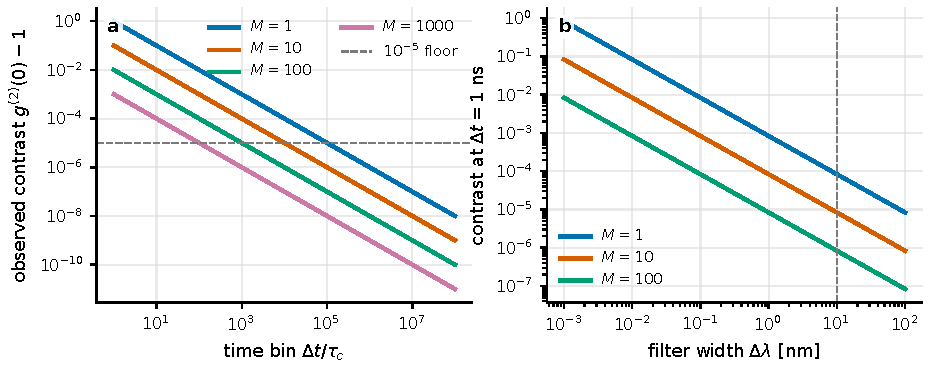
\includegraphics[width=0.96\linewidth]{figures/generated/chapter_21/ch21_g2_scaling_mistake.pdf}
\caption{How the time bin, spectral bandwidth, and mode number dilute the contrast of \(g^{(2)}\). The left panel shows how \(\Delta t/\tau_c\) and \(M_{\rm eff}\) press the bunching peak of single-mode thermal light down; the dashed line marks the \(10^{-5}\)-level systematic-error floor. The right panel converts the filter bandwidth into coherence time: at \(1\,{\rm ns}\) sampling, the thermal peak of broadband visible light easily falls below the calibratable range. This is precisely the true origin of ``\(g^{(2)}\simeq1\)'': not the absence of quantum nature, but the quantum nature being averaged and diluted away.}
\label{fig:e27-g2-scaling}
\end{figure}

Then what is a \textbf{truly ironclad nonclassical criterion}? The answer is antibunching, that is,
\[
  g^{(2)}(0)<1.
\]
Chapter \ref{chap:e08} proved: any classical random intensity satisfies \(g^{(2)}(0)\ge1\) (a direct consequence of the Cauchy--Schwarz inequality), so \(g^{(2)}(0)<1\) is something classical light \emph{can never do}: it means photons ``avoid'' one another, the signature of a single quantum emitter. The resonance-fluorescence experiment of Kimble, Dagenais, and Mandel first firmly established antibunching precisely by measuring \(g^{(2)}(0)<1\) \citep{1977PhRvL..39..691K}. But seeing antibunching in astronomical light sources is nearly impossible: the light of an object is usually the result of a vast number of independent emitters, countless propagation paths, and finite detector response all mixed together, and any sub-Poisson feature of a single quantum emitter is diluted beyond visibility by that enormous \(M_{\rm eff}\) in Eq.\ \eqref{eq:e27-dilution}.

So the lesson of this section is bidirectional: an astronomical report that writes ``\(g^{(2)}\simeq1\), therefore this is a laser,'' or writes ``\(g^{(2)}\simeq1\), therefore there is no quantum information,'' has no basis for either statement. \(\mathbf{g^{(2)}\simeq1}\) \textbf{is the default result after dilution; it neither proves coherence nor disproves quantumness; only }\(\mathbf{g^{(2)}(0)<1}\)\textbf{ is incontrovertible nonclassical evidence.}


\section{Why intensity interferometry still cannot do without calibration}
\label{sec:e27-calibration}

The third pitfall arises from over-optimism about a real advantage of intensity interferometry. Chapter \ref{chap:e10} explained that intensity interferometry measures the correlation of two intensity-fluctuation streams, and is insensitive to the overall atmospheric phase (piston, the common shift phase of the two paths' optical lengths): this is its greatest engineering advantage over amplitude interferometry, and the reason Hanbury Brown and Twiss could measure stellar angular diameters at Narrabri with crude mirrors \citep{1956Natur.178.1046H,1957RSPSA.242..300B,1974iiia.book.....H}. But ``not fearing phase'' is easily misread as ``not fearing error.'' The truth is exactly the opposite: because the signal sought has already been diluted to the \(10^{-5}\) level (previous section), any \emph{amplitude} error of the same order can overturn the conclusion.

Write the actually measured excess correlation as a data model, and one sees which terms are making trouble:

\begin{equation}
  \hat c_b(\tau)=
  \beta_b\,|V_b|^2\,h_b(\tau)
  +c_{{\rm inst},b}(\tau)
  +c_{{\rm sel},b}(\tau)
  +\epsilon_b(\tau).
  \label{eq:e27-calibration-model}
\end{equation}
\begin{formulaexplain}
\(\hat c_b=\hat g_b^{(2)}-1\) is the normalized excess correlation measured on baseline \(b\). The first term is the true astronomical signal, followed in order by the instrument term, the selection term, and the random error. Intensity interferometry does not fear atmospheric \emph{phase}, but it fears these \emph{amplitude} terms just the same.
\end{formulaexplain}

Taking each term apart, all quantities are dimensionless correlation amplitudes. \(\hat c_b\) is the normalized excess measured on baseline \(b\) (a pair of telescopes, one delay segment); \(\beta_b\) is the zero-baseline contrast or instrument dilution factor, precisely the concrete embodiment of that \(1/M_{\rm eff}\) in Eq.\ \eqref{eq:e27-dilution}; \(|V_b|^2\) is the square of the object's visibility, carrying the angular-scale information; \(h_b(\tau)\) is the normalized peak shape. The real trouble is in the last three terms: \(c_{\rm inst}\) is the spurious correlation brought by the electronics and detector: electronic crosstalk, photomultiplier gain drift, SPAD dead time, TDC (time-to-digital converter) quantization spurious peaks; \(c_{\rm sel}\) is the term caused by the selection function, weather, and background processing; and \(\epsilon\) is the random noise. VERITAS explicitly handles background light and zero-baseline correlation when fitting stellar angular diameters, and MAGIC's real-time correlator is designed around continuous recording, low crosstalk, and fast mode switching \citep{2020NatAs...4.1164A,2024MNRAS.529.4387A,2024ApJ...966...28A}.

Here is an especially deadly misconception: \textbf{believing that as long as one integrates long enough, systematic error will be pushed down}. It will not. The random error \(\epsilon\) does shrink as \(T^{-1/2}\) with integration time \(T\): integrate ten thousand times as long and the random error falls a hundredfold. But \(c_{\rm inst}\) and \(c_{\rm sel}\) in Eq.\ \eqref{eq:e27-calibration-model} are \emph{systematic} terms; they do not decay with \(T\), but only form a ``systematic-error floor.'' Once the random error falls to the floor height (usually \(10^{-5}\)--\(3\times10^{-5}\) for current experiments), continuing to integrate no longer improves the conclusion: the curve \emph{saturates}. The left of Figure \ref{fig:e27-calibration} draws an electronic-crosstalk peak more than an order of magnitude above a \(5\times10^{-5}\) astronomical bunching peak, and the right draws the saturation after the integration curve hits the floor.

\begin{figure}[tbp]
\centering
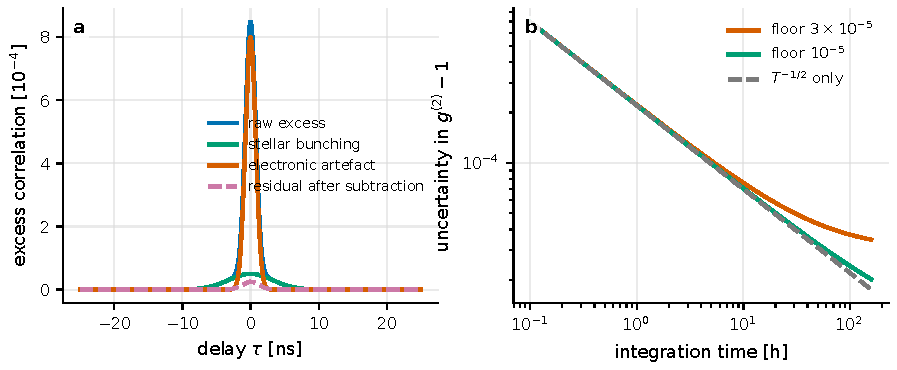
\includegraphics[width=0.96\linewidth]{figures/generated/chapter_21/ch21_calibration_artifacts.pdf}
\caption{How calibration errors disguise themselves as correlation signal. In the left panel an electronic-crosstalk peak is more than an order of magnitude above a \(5\times10^{-5}\) astronomical bunching peak; if a narrow residual remains after template subtraction, it contaminates \(\hat g^{(2)}(0)\). The right panel shows that integration time only presses down the \emph{statistical} error as \(T^{-1/2}\); once a systematic floor of \(10^{-5}\)--\(3\times10^{-5}\) exists, more integration cannot automatically improve the conclusion.}
\label{fig:e27-calibration}
\end{figure}

The correct stance against systematic terms is not ``integrate longer'' but to design a whole suite of null tests, making ``true signal'' and ``spurious signal'' behave differently under different operations: a time-shift moves one stream's events as a whole by a time far greater than the correlation width, and the true astronomical peak should vanish, while slow drift and background structure should remain; off-source or off-band switches the field or frequency band to a place without the target, and the zero-delay peak should not remain; channel permutation cross-correlates detectors, polarizations, or spectral channels that should not be correlated, and if a peak persists, suspect crosstalk first; block convergence slices the data into segments, and the mean of the correlation amplitude should be stable and the error should fall as \(T^{-1/2}\) \emph{until} it hits the floor. Guerin's report points out that if the TDC spurious correlation is not subtracted, the signal-to-noise saturates prematurely; the AQuEye/IquEye literature also explicitly lists the contributions of SPAD dead time, fiber delay, and environmental control to systematic error \citep{2017MNRAS.472.4126G,2016SPIE.9907E..0NZ,1996ApOpt..35.1956C,2013NIMPA.725..187J,2020RScI...91a3108W}.

To close: \textbf{what intensity interferometry spares you is atmospheric phase, not calibration; since the signal is diluted to }\(\mathbf{10^{-5}}\)\textbf{, one must assume instrument spurious correlations of the same order are always present, and deal with them by null tests rather than longer integration.}


\section{Why ``no phase'' does not mean ``cannot image''}
\label{sec:e27-phase}

The fourth pitfall comes from a sentence that sounds very reasonable: ``Intensity interferometry loses the phase, so it can only measure diameters, not image.'' The first half is right, the second half is wrong.

First state the right part clearly. The van Cittert--Zernike theorem of Chapter \ref{chap:e10} tells us that the angular Fourier transform of the object's brightness distribution \(I(\boldsymbol\theta)\) is the complex visibility \(V(u,v)\), which has both modulus and phase. Amplitude interferometry directly measures this complex \(V\); intensity interferometry measures the correlation of two intensity streams and obtains the modulus squared \(|V(u,v)|^2\), and \textbf{the phase of the first-order complex visibility is indeed lost}. This is a real loss of information and cannot be pretended away.

But ``losing the phase'' by no means equals ``no structure can be measured.'' \(|V|^2\) still contains a great deal of information: the diameter of a uniform disk, the degree of limb darkening, the separation and brightness ratio of a binary, the ellipticity of a rotationally flattened star, the scale of a simple disk: all can be directly fit from the dependence of \(|V|^2\) on \(u,v\). Chapter \ref{chap:e11}, in going from visibility to imaging, does exactly this. The real difficulty losing the phase brings is a specific class of \textbf{degeneracy}, the cleanest of which is the mirror degeneracy.

The reasoning of the mirror degeneracy can be laid bare in one line of algebra. Imagine reflecting the brightness distribution through a point inversion, \(I(\boldsymbol\theta)\to I(-\boldsymbol\theta)\). The Fourier transform has a basic property: if a function is point-inverted, its spectrum is complex-conjugated. Denote the complex visibility of the original brightness \(I(\boldsymbol\theta)\) as \(V(\boldsymbol u)\) (i.e.\ \(V=\widetilde I\)); then the inverted brightness \(I(-\boldsymbol\theta)\) has visibility
\[
  \mathcal V_{I(-\boldsymbol\theta)}(\boldsymbol u)
  \equiv\widetilde{I(-\boldsymbol\theta)}(\boldsymbol u)
  =V^\ast(\boldsymbol u).
\]
Taking the modulus squared,
\[
  \big|\mathcal V_{I(-\boldsymbol\theta)}(\boldsymbol u)\big|^2
  =\big|V^\ast(\boldsymbol u)\big|^2=\big|V(\boldsymbol u)\big|^2.
\]
The two are \emph{completely identical}. This means: an object and its mirror image produce the exact same \(|V|^2\), and intensity interferometry \emph{in principle} cannot separate them: the orientation information needed to separate the two is hidden precisely in the discarded sign of the visibility phase. Chapter \ref{chap:e11} already drew this phase-loss problem; Figure \ref{fig:e27-phase-loss} demonstrates it again with an unequal-brightness double source and its mirror image.

\begin{figure}[tbp]
\centering
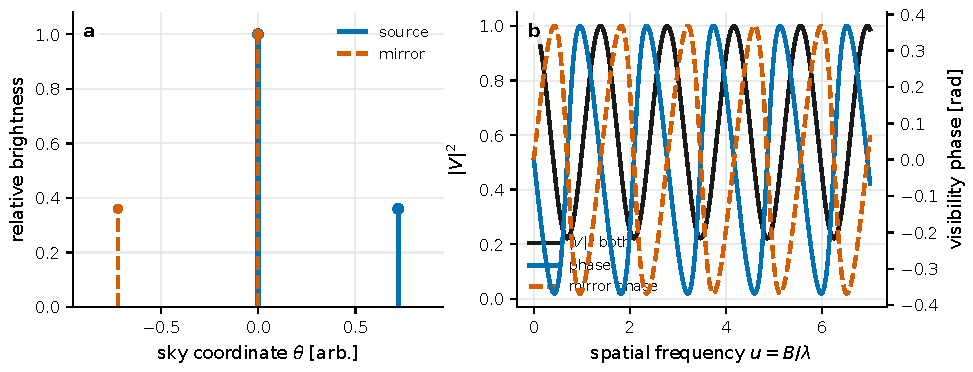
\includegraphics[width=0.96\linewidth]{figures/generated/chapter_21/ch21_phase_loss.pdf}
\caption{The mirror degeneracy from measuring only \(|V|^2\). The left panel is an unequal-brightness double source and its point-inverted mirror image; the right panel shows that the \(|V|^2\) of the two completely overlap, differing only in the sign of the visibility phase. Intensity interferometry can constrain structure, but to recover the lost orientation information one must rely on multi-baseline coverage, model priors, or higher-order correlation.}
\label{fig:e27-phase-loss}
\end{figure}

To distinguish mirror images, asymmetric structures, and complex morphologies, the correct approach is not to complain ``no phase'' but to add information: spread out multiple baselines, add physical priors, use regularized phase retrieval, or introduce higher-order information such as third-order intensity correlation \citep{2003RPPh...66..789M,2009A&A...507.1719F,2012NewAR..56..143D,2014MNRAS.437..798M,2022MNRAS.512.1722K}. The third-order correlation deserves a separate word, because it is often over-promised: ideally, third-order intensity correlation can give closure-phase-like information, thereby partially recovering orientation; but its signal is \emph{weaker} than the second-order correlation. If the statistical error of the second-order correlation is already against the systematic floor of the previous section, the third-order correlation is pinned even harder by the same photon rate and the same set of calibration problems. So third-order correlation is an exploratory direction for large arrays and extremely bright targets, while first-generation science cases (Chapter \ref{chap:e25}) are usually more pragmatic: start from few-parameter models of \(|V|^2\), then gradually add priors to build up imaging.

To close: \textbf{what intensity interferometry loses is the visibility \emph{phase}, not all structure;} \(\mathbf{|V|^2}\)\textbf{ suffices to constrain diameter, binaries, ellipticity, and many other quantities; what is truly lost is the orientation information distinguishing mirror images, to be recovered by multiple baselines, priors, or higher-order correlation.}


\section{Why quantum super-resolution cannot arbitrarily break diffraction}
\label{sec:e27-superres}

The fifth pitfall grows right beside a real achievement, so it is especially easy to fall into. SPADE (spatial-mode demultiplexing) corrects a genuine statistical misunderstanding: \textbf{the Rayleigh criterion is not the information limit of all parameter-estimation problems}. Chapter \ref{chap:e12} proved, without skipping a step: for two faint, equal-brightness, mutually incoherent point sources, when the angular separation \(s\) is far smaller than the point-spread-function width \(\sigma\), the Fisher information of direct imaging about \(s\) falls to zero as \(s^2\) (the so-called ``Rayleigh curse''), while ideal spatial-mode sorting can keep the per-photon Fisher information at a finite value \citep{2015Optic...2..646T,2016PhRvX...6c1033T,2016OExpr..24.3684N,2017PhRvL.118g0801T}. This is a true conclusion; do not discount it.

But precisely because it is true, one must all the more guard against its being exaggerated into ``quantum super-resolution can arbitrarily break diffraction, and reconstruct any complex image from a few photons.'' To see the boundary clearly, return to the Cramér--Rao bound of Chapter \ref{chap:e12}. The variance of any unbiased estimator \(\hat s\) satisfies
\begin{equation}
  \operatorname{Var}(\hat s)\;\ge\;\frac{1}{N_\gamma\,F_s},
  \label{eq:e27-crb}
\end{equation}
\begin{formulaexplain}
\(\hat s\) is the estimate of the angular separation, \(N_\gamma\) is the number of photons entering the correct mode analysis, and \(F_s\) is the Fisher information \emph{per photon} about \(s\). The measurement mode can change \(F_s\) but not \(N_\gamma\); to truly attain the bound, there must moreover be no background, aberration, or mode crosstalk.
\end{formulaexplain}

Ground each symbol. \(s\) is the angular separation to be estimated, in units of rad, mas, or directly normalized by the PSF width \(\sigma\); \(N_\gamma\) is the dimensionless effective photon number: note it is the number of photons that \emph{entered the correct mode analysis}, not the total photons hitting the telescope; \(F_s\) is the per-photon Fisher information, with dimensions of angle to the power \(-2\). Equation \eqref{eq:e27-crb} makes three things clear at once: first, what SPADE raises is \(F_s\) (blocking the \(s^2\to0\) collapse), and it \textbf{cannot substitute for }\(N_\gamma\): if the photons are too few, the variance blows up anyway; second, the bound is a ``\(\ge\),'' the \emph{best} achievable case, and \textbf{the quantum bound is not automatically attainable}: background, aberration, mode crosstalk, and centroid error each make the actual variance higher than this line; third, carrying the two-point conclusion over to an arbitrary complex image has no basis. The left of Figure \ref{fig:e27-superresolution} draws mode sorting indeed pulling the error scale far down, but a mode/centroid error floor of \(0.003\sigma\)--\(0.01\sigma\) stops the improvement; the right, with a toy model, shows that to recover higher-order moments or modes, the required photon number rises \emph{sharply}.

\begin{figure}[tbp]
\centering
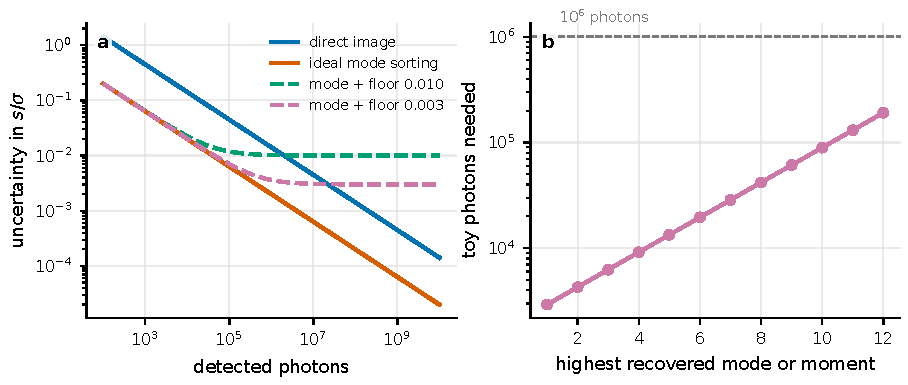
\includegraphics[width=0.96\linewidth]{figures/generated/chapter_21/ch21_superresolution_budget.pdf}
\caption{The photon budget and systematic floor of quantum super-resolution. The left panel takes \(s=0.2\sigma\) and compares the statistical-error scale of direct imaging and ideal mode sorting: mode sorting markedly lowers the error, but a mode/centroid error floor of \(0.003\sigma\)--\(0.01\sigma\) makes the improvement stop. The right panel, with a toy model, shows that the photon number required to recover higher-order moments or modes rises rapidly: a complex image cannot be arbitrarily recovered from a few photons.}
\label{fig:e27-superresolution}
\end{figure}

In the astronomical context there is a finer condition often overlooked: the coherence of the source itself, and the first-order spatial coherence after propagation. SPADE's clean conclusion is proved for ``two \emph{mutually incoherent} Gaussian point sources''; once the source is partially coherent, the mode probabilities change, and whether the Rayleigh curse reappears is precisely the condition around which the field's discussion revolves \citep{2017NJPh...19b3054T,2017PhRvA..95f3847A,2018Optic...5.1177P,2018Optic...5.1382L,2019Optic...6..400T}. Therefore, carrying the ``two incoherent Gaussian sources'' conclusion directly over to galaxies, accretion disks, jets, or strong-lensing arcs quietly discards the conditions of applicability.

To close: \textbf{the Rayleigh criterion is not the estimation limit: this is SPADE's real substance; but the quantum bound in Eq.\ }\eqref{eq:e27-crb}\textbf{ both needs sufficient }\(\mathbf{N_\gamma}\)\textbf{ and is not automatically attainable, and stripped of the conditions ``two-point, incoherent, no background, mode-aligned,'' super-resolution is only a slogan.}


\section{Where astrophysical lasers, masers, and non-Poisson statistics are most easily confused}
\label{sec:e27-maser}

The sixth pitfall centers on astrophysical stimulated-emission sources, and is several misunderstandings twisted together. The most typical line is: ``An astrophysical laser/maser must give \(g^{(2)}=1\).''

First unravel the first layer: \textbf{high brightness temperature does not equal a coherent state}. Stimulated emission can produce extremely high brightness temperature, extremely narrow spectral lines, and very strong polarization: these are the trademarks of a maser (microwave amplification by stimulated emission of radiation). But the trademark is not the intrinsic statistics. A laboratory laser approaches a coherent state by relying on a stable resonant cavity plus saturated gain to clamp the intensity fluctuations; an astrophysical environment has no such cavity at all. Chapter \ref{chap:e06} made the distinction: a coherent state is a very special quantum state, whose fingerprint is a \emph{Poisson} photon-number distribution, not ``bright'' or ``narrow.'' A spectral line that is both bright and narrow may perfectly well still carry strong intensity fluctuations: brightness temperature, line width, and polarization are measures of ``how bright, how narrow, how orderly,'' while photon statistics is a measure of ``how large the fluctuations are''; the two yardsticks measure different things. Unsaturated masers, saturated masers, velocity-coherent paths, pump fluctuations, superposition of multiple spots, and continuum background each rewrite the photon statistics \citep{1982RvMP...54.1225E,1992ARA&A..30...75E,1985ARA&A..23..169D}. In the Weigelt blobs of Eta Carinae, the natural-laser candidates of the Fe II and O I lines can be characterized only by simultaneously examining Ly\(\alpha\) pumping, level inversion, line width, spatial position, and continuum subtraction; a Brown--Twiss--Townes heterodyne correlation has even been proposed specifically to measure the line width of that extremely narrow Fe II line \citep{2004A&A...428..497J,2005MNRAS.364..731J,2005NewA...10..361J,2008AIPC..984..216D}.

The second layer is mixture dilution, worth deriving without skipping a step. Suppose the observed light is the superposition of several independent components, total intensity \(I=\sum_a I_a\), with no intensity correlation between different components. The zero-delay second-order coherence is
\[
  g^{(2)}_{\rm mix}(0)=\frac{\langle I^2\rangle}{\langle I\rangle^2}.
\]
First compute the numerator. Expand \(I^2=\big(\sum_a I_a\big)^2=\sum_a I_a^2+\sum_{a\ne b}I_aI_b\), and take the average:
\[
  \langle I^2\rangle
  =\sum_a\langle I_a^2\rangle
  +\sum_{a\ne b}\langle I_a\rangle\langle I_b\rangle,
\]
where the cross term used the assumption ``no correlation between different components,'' splitting \(\langle I_aI_b\rangle\) into \(\langle I_a\rangle\langle I_b\rangle\). Then use each component's own definition \(\langle I_a^2\rangle=g_a^{(2)}(0)\langle I_a\rangle^2\), and complete the cross sum into a full double sum minus the diagonal:
\[
  \sum_{a\ne b}\langle I_a\rangle\langle I_b\rangle
  =\Big(\sum_a\langle I_a\rangle\Big)^2-\sum_a\langle I_a\rangle^2
  =\langle I\rangle^2-\sum_a\langle I_a\rangle^2.
\]
Together:
\[
  \langle I^2\rangle
  =\sum_a g_a^{(2)}(0)\langle I_a\rangle^2
  +\langle I\rangle^2-\sum_a\langle I_a\rangle^2.
\]
Divide both sides by \(\langle I\rangle^2\), and denote the flux fraction \(f_a=\langle I_a\rangle/\langle I\rangle\):
\[
  g^{(2)}_{\rm mix}(0)
  =\sum_a g_a^{(2)}(0)f_a^2+1-\sum_a f_a^2.
\]
Move the 1 to the left, combine the right by \(f_a^2\), and obtain the clean result:

\begin{equation}
  g^{(2)}_{\rm mix}(0)-1
  =\sum_a f_a^2\left[g_a^{(2)}(0)-1\right],
  \qquad
  f_a=\frac{\langle I_a\rangle}{\sum_b\langle I_b\rangle}.
  \label{eq:e27-mixture}
\end{equation}
\begin{formulaexplain}
\(f_a\) is the flux fraction of the \(a\)-th component (dimensionless, summing to 1 over components). The crux is that \emph{square}: the correlation excess is weighted by \(f_a^2\), so a little bit of thermal continuum or multi-component mixture can scramble the reading of \(g^{(2)}\).
\end{formulaexplain}

That square is the whole crux. Plug in a number: a thermal component making up only \(20\%\) of the total flux, even if it is at full-scale \(g_a^{(2)}(0)-1=1\) on its own, contributes after mixing only \(f_a^2\times1=0.2^2=0.04\) of contrast; if this thermal component is further spread over \(M=100\) modes with \(\tau_c/\Delta t=10^{-5}\), the observed contrast becomes \(0.04\times10^{-5}/100\sim4\times10^{-9}\), completely sunk to the bottom. Conversely, an unsaturated stimulated line carrying pump intensity noise may give \emph{super}-Poisson statistics; but such a result must first cleanly separate the line, the continuum, and the instrument response, and one must never attribute \(g^{(2)}>1\) to new physics on sight. Figure \ref{fig:e27-maser} draws these two branches together.

\begin{figure}[tbp]
\centering
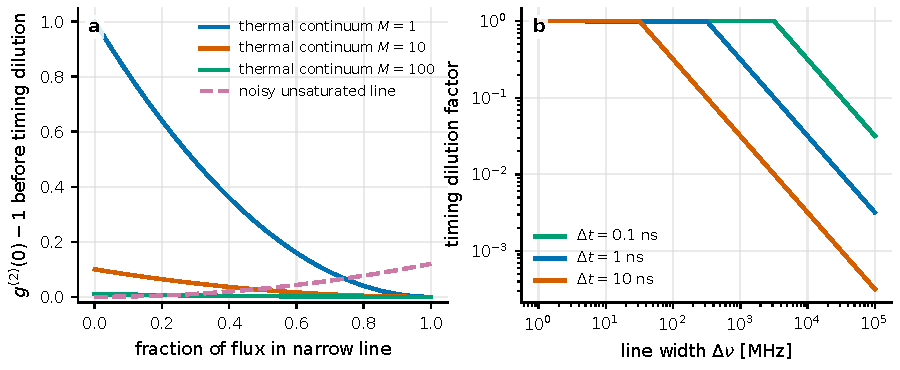
\includegraphics[width=0.96\linewidth]{figures/generated/chapter_21/ch21_maser_mixed_statistics.pdf}
\caption{Mixed statistics in astrophysical maser/laser candidates. The left panel shows that as the narrow-line flux fraction increases, the bunching of the thermal continuum is diluted by \(f_a^2\); if the narrow line itself carries unsaturated intensity noise, another super-Poisson branch emerges. The right panel shows the dilution of the correlation contrast by the line width and the electronics time bin: an MHz--GHz line width requires a ns or even faster time response to preserve an appreciable peak.}
\label{fig:e27-maser}
\end{figure}

The third layer: non-Poisson statistics have far too many \emph{ordinary} sources; do not rush to attribute them to a quantum light source. The most typical is treating a randomly variable source as a Cox process (a Cox process, also called a doubly stochastic Poisson process): given an instantaneous rate \(\Lambda\), the count is Poisson, but \(\Lambda\) itself fluctuates with time or environment. Using the law of total variance (splitting the variance into ``the expectation of the conditional variance'' plus ``the variance of the conditional expectation''), denoting \(\Lambda\) as the expected count in a bin, with Poisson conditions \(\operatorname{Var}(N\mid\Lambda)=\Lambda\) and \(\mathbb E(N\mid\Lambda)=\Lambda\), we have
\[
  \operatorname{Var}(N)
  =\mathbb E[\operatorname{Var}(N\mid\Lambda)]+\operatorname{Var}(\mathbb E[N\mid\Lambda])
  =\mathbb E(\Lambda)+\operatorname{Var}(\Lambda),
\]
while \(\mathbb E(N)=\mathbb E(\Lambda)\). Dividing the two gives the Fano factor:

\begin{equation}
  F_{\rm Fano}
  \equiv\frac{\operatorname{Var}(N)}{\mathbb E(N)}
  =1+\frac{\operatorname{Var}(\Lambda)}{\mathbb E(\Lambda)}.
  \label{eq:e27-fano}
\end{equation}
\begin{formulaexplain}
\(F_{\rm Fano}\) is the ratio of count variance to mean (equal to 1 for pure Poisson). As long as the instantaneous rate \(\Lambda\) itself fluctuates, the count naturally becomes super-Poisson (\(F>1\)), with no need to invoke a nonclassical light source at all.
\end{formulaexplain}

That is, as long as the source varies, \(F_{\rm Fano}\) at a suitable bin width is \emph{necessarily} greater than 1: the most trivial super-Poisson. The instrument also makes trouble from the opposite direction: dead time suppresses events too close together, producing negative correlation at short delays and pressing \(F_{\rm Fano}\) below 1 (under-dispersion); afterpulsing produces positive correlation after the detector's characteristic time. The afterpulsing probability of \(10^{-4}\)--\(10^{-2}\) given in Chapter \ref{chap:e07} is already enough to contaminate many short-delay searches. So before shouting ``non-Poisson,'' first draw the full set of diagnostic plots: the Fano factor versus bin width, the short-delay auto- and cross-correlation, dark-field data, off-source data, and the time-shift background. Figure \ref{fig:e27-nonpoisson} draws the different scalings of these ordinary sources side by side.

\begin{figure}[tbp]
\centering
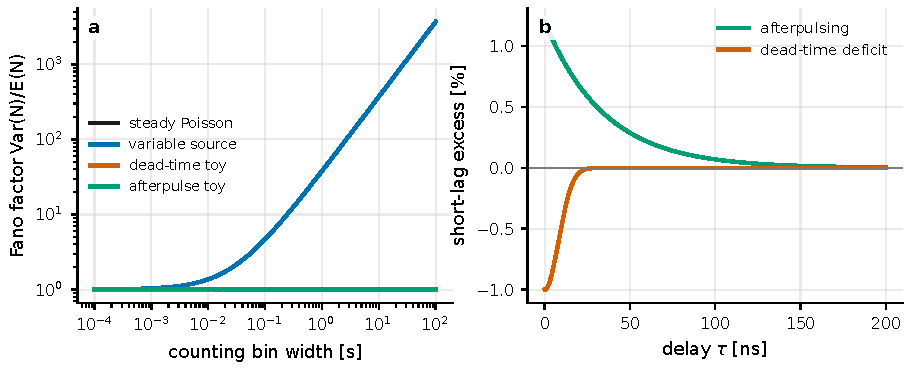
\includegraphics[width=0.96\linewidth]{figures/generated/chapter_21/ch21_nonpoisson_diagnostics.pdf}
\caption{Ordinary sources of non-Poisson statistics. The left panel uses the Fano factor to display the distinct scalings of steady-state Poisson, a slowly varying source, dead time, and afterpulsing: a slowly varying source becomes super-Poisson in long bins, and dead time causes under-dispersion. The right panel shows the opposite shapes of afterpulsing and dead time in the short-delay correlation function: these instrument features should first be quantified from dark-field and cross-channel data.}
\label{fig:e27-nonpoisson}
\end{figure}

To close: \textbf{bright, narrow, and strongly polarized do not equal a coherent state; mixed light dilutes the correlation by }\(\mathbf{f_a^2}\)\textbf{, and variable sources, dead time, and afterpulsing naturally manufacture non-Poisson statistics: before they are cleanly ruled out, no ``non-Poisson'' should be charged to new physics.}


\section{How false alarms fabricate the boundary of ``new physics''}
\label{sec:e27-false-alarm}

The last pitfall is the common ailment of all search-type work: mistaking one low-probability event for a discovery.

The root of the problem is ``multiple testing.'' Suppose the tail probability of one test giving a result this extreme by chance is \(p_0\), and you independently do \(N_{\rm trial}\) tests; then what is the probability of ``at least one'' such chance peak? Step by step: the probability of a single test \emph{not} occurring is \(1-p_0\), all \(N_{\rm trial}\) tests not occurring is \((1-p_0)^{N_{\rm trial}}\) (using independence of each), so at least one occurring is

\begin{equation}
  p_{\rm any}=1-(1-p_0)^{N_{\rm trial}}
  \simeq N_{\rm trial}\,p_0
  \qquad(N_{\rm trial}\,p_0\ll1).
  \label{eq:e27-trials}
\end{equation}
\begin{formulaexplain}
\(p_0\) is the tail probability of a single test, and \(N_{\rm trial}\) is the number of trials. The larger the search space, the higher the probability of chancing upon a high peak, so one must report the \emph{global} significance, not the single \(p_0\).
\end{formulaexplain}

That approximate equality comes from one step of standard expansion: when \(p_0\) is very small \emph{and} \(N_{\rm trial}p_0\ll1\), \((1-p_0)^{N_{\rm trial}}\approx e^{-N_{\rm trial}p_0}\approx1-N_{\rm trial}p_0\) (first using \(\ln(1-p_0)\approx-p_0\), then a first-order Taylor expansion of the exponential), and substituting back gives \(p_{\rm any}\approx N_{\rm trial}p_0\). One must remember this approximation \textbf{holds only when }\(\mathbf{N_{\rm trial}p_0\ll1}\); once the search space is so large that \(N_{\rm trial}p_0\gtrsim1\), it can no longer be used, and one must return to the un-approximated \(p_{\rm any}=1-(1-p_0)^{N_{\rm trial}}\approx1-e^{-\mu}\), where we denote
\[
  \mu\equiv N_{\rm trial}\,p_0
\]
as the \textbf{expected number} of chance peaks (dimensionless, and can be far greater than 1), while the probability \(p_{\rm any}=1-e^{-\mu}\) always lies between \(0\) and \(1\). This \(N_{\rm trial}\) can arise from all directions: the number of time bins, frequency channels, baselines, targets, model-grid points, and even windows circled out only after the fact. Plug in a number to feel it: if each night one scans \(10^6\) candidate delay/frequency/target combinations, an event with single \(p_0=10^{-5}\) (which sounds ``very significant'' already) has an expected number of chance peaks
\[
  \mu=N_{\rm trial}\,p_0\simeq10^{6}\times10^{-5}=10,
\]
so the probability of occurring globally is
\[
  p_{\rm any}=1-e^{-\mu}\approx1-e^{-10}\approx0.99995\approx1,
\]
nearly certain: meaning about \(\mu\approx10\) such ``astonishing peaks'' emerge each night on average, purely the natural tail of the search space. Here one must sharply distinguish two things: \(10\) is the expected \emph{number} \(\mu\), not a probability; writing it as \(p_{\rm any}=10\) (and casually forcing the approximation \(p_{\rm any}\approx N_{\rm trial}p_0\), which holds only for \(\mu\ll1\), onto \(\mu=10\)) is exactly the typical error this section teaches you to avoid: a probability can never exceed 1, and the quantity exceeding 1 must be the expected value of a count. The left of Figure \ref{fig:e27-false-alarm} draws a single Poisson bin with \(\mu=8\) occasionally flinging out a high-count tail of \(N\ge17\), and the right draws how the same single \(p_0\) rolls, after many trials, into a very high global false-alarm probability.

\begin{figure}[tbp]
\centering
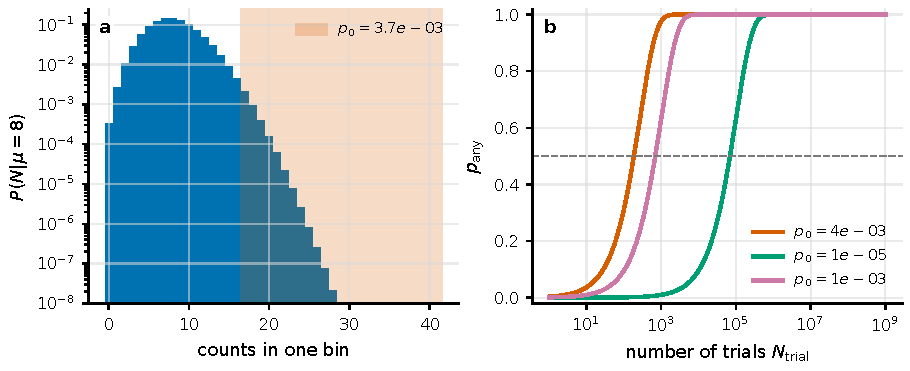
\includegraphics[width=0.96\linewidth]{figures/generated/chapter_21/ch21_poisson_false_alarm.pdf}
\caption{Poisson tails and multiple testing. In the left panel a single bin with \(\mu=8\) occasionally shows a high-count tail of \(N\ge17\); the right panel shows how the same single \(p_0\) becomes a very high global false-alarm probability over many trials. Event-table searches, period searches, cross-frequency correlations, and transient screening must all report \(N_{\rm trial}\) or the equivalent global significance.}
\label{fig:e27-false-alarm}
\end{figure}

Along the way, correct a larger semantic misunderstanding: \textbf{``quantum astronomy'' does not equal ``quantum gravity.''} The vast majority of the book so far studies light-field statistics, mode measurement, coherence functions, instruments, and information limits: all measurable ground physics. Black holes, the CMB, axions, cosmic birefringence, and dark-matter lensing can enter this main line because they can be written as \emph{observable} temporal, frequency, polarization, or spatial correlation quantities, not because each topic must invoke Planck-scale physics. The first step of a genuinely checkable anomaly is always to decompose the data sources:
\begin{equation}
  d_{\rm obs}=d_{\rm sky}(\boldsymbol\theta)
  +d_{\rm inst}(\boldsymbol\phi)
  +d_{\rm sel}(\boldsymbol\psi)
  +n.
  \label{eq:e27-data-model}
\end{equation}
\begin{formulaexplain}
\(d_{\rm obs}\) is the observed data (delay histogram, \(|V|^2\), polarization correlation, or event times); the right side separates the sky model, the instrument model, the selection function, and the noise. Any ``new physics'' explanation must first prove that these preceding ordinary terms \emph{cannot} explain the data.
\end{formulaexplain}

Here \(d_{\rm sky}(\boldsymbol\theta)\) is the object model (parameters \(\boldsymbol\theta\)), \(d_{\rm inst}(\boldsymbol\phi)\) is the instrument model, \(d_{\rm sel}(\boldsymbol\psi)\) is the selection function, and \(n\) is the noise. As long as these four terms are not yet separated, an anomalous peak, polarization rotation, or super-Poisson count should not be directly attributed to new physics; they more likely hide in \(d_{\rm inst}\) or \(d_{\rm sel}\). This connects neatly to Chapter \ref{chap:e28}: the last page of a research plan should return to ``what exactly is the new observable'': average intensity, second-order correlation, cross-frequency covariance, polarization correlation, or mode count; each quantity must come with units, typical range, and conditions of applicability (thermal light, Gaussian PSF, faint light, few-parameter source model, stable instrument response), and pick at least two null tests from time shift, off-source, off-band, dark field, wrong polarization, and injection-recovery, writing the global significance and the systematic-error floor \emph{together} into the conclusion.

To close: \textbf{the larger the search space, the more inevitable an accidental ``significant peak''; a significance that does not report }\(\mathbf{N_{\rm trial}}\)\textbf{ is meaningless, and the threshold of ``quantum astronomy'' is an observable correlation quantity, not new Planck-scale physics.}


\section{Chapter Summary}
\label{sec:e27-summary}

\begin{itemize}
  \item \textbf{Counting photons only obtains the raw material.} The real quantum information is in the joint distribution among events; if the time, detector, frequency, and polarization labels do not enter the model, even the most precise single-photon counting is still classical photometry. ``Few photons'' and ``quantum'' are two different yardsticks.
  \item \(\mathbf{g^{(2)}\simeq1}\)\textbf{ proves nothing.} The bunching peak of thermal light being diluted by the effective mode number \(M_{\rm eff}\) (including \(\Delta t_{\rm eff}/\tau_c\)) to \(10^{-5}\)--\(10^{-6}\) is the norm, see Eq.\ \eqref{eq:e27-dilution}. The only ironclad nonclassical criterion is antibunching \(g^{(2)}(0)<1\), which classical light cannot do.
  \item \textbf{Intensity interferometry does not fear phase, but fears calibration.} Since the signal is diluted to \(10^{-5}\), one must assume instrument spurious correlations of the same order are always present (Eq.\ \eqref{eq:e27-calibration-model}). The systematic floor does not fall as \(T^{-1/2}\); deal with it by null tests, not longer integration.
  \item \(\mathbf{|V|^2}\)\textbf{ loses the phase, not the structure.} Diameter, binaries, and ellipticity can all be fit; what is truly lost is the orientation information distinguishing mirror images (\(|V^\ast|^2=|V|^2\)), to be recovered by multiple baselines, priors, or higher-order correlation.
  \item \textbf{Quantum super-resolution has boundaries.} The Rayleigh criterion is indeed not the estimation limit, but the quantum bound of Eq.\ \eqref{eq:e27-crb} both needs sufficient photons \(N_\gamma\) and is not automatically attainable; away from ``two-point, incoherent, no background, mode-aligned'' it is only a slogan.
  \item \textbf{Bright, narrow, strongly polarized does not equal a coherent state.} Mixed light dilutes the correlation by \(f_a^2\) (Eq.\ \eqref{eq:e27-mixture}), and variable sources (Cox process, Eq.\ \eqref{eq:e27-fano}), dead time, and afterpulsing all naturally manufacture non-Poisson statistics: not new physics until cleanly ruled out.
  \item \textbf{A search must report global significance.} Chance peaks increase linearly with \(N_{\rm trial}\) (Eq.\ \eqref{eq:e27-trials}); an anomaly must first be decomposed into the four terms sky/instrument/selection/noise (Eq.\ \eqref{eq:e27-data-model}) before new physics can be discussed.
\end{itemize}

\medskip
\noindent\textbf{Questions to Ponder.}
\begin{itemize}
  \item You measure the thermal light of a star at \(500\,{\rm nm}\), \(5\,{\rm nm}\) bandwidth, with a \(2\,{\rm ns}\) correlation bin. In the single-mode case, what order of magnitude of \(g^{(2)}_{\rm meas}(0)-1\) do you expect to measure? (Hint: first compute \(\tau_c\), then use Eq.\ \eqref{eq:e27-dilution}.)
  \item In a spectral-line search, you find in \(3\times10^{5}\) frequency channels a peak with single \(p_0=3\times10^{-6}\). What is its global false-alarm probability? Would you declare a discovery?
  \item Someone reports \(g^{(2)}(0)=1.5\) for an astrophysical maser, claiming it is nonclassical light. Before believing it, which three ordinary sources would you first require them to rule out?
\end{itemize}
